\chapter{Audio Signal Processing and Inverse Problem}\label{ch:processing}
% \openepigraph{Sound, a certain movement of air.}{Aristotele, De Anima II.8 420b12}
\vspace{-2.5em}
\newthought{Synopsis} Let us now move from the physic to digital signal processing.
This chapter formalizes the concept of mixtures of audio signals and the concept of audio inverse problems.
\\The chapter defines and discusses the signal model~\cref{sec:processing:model}.

\section{Definitions and signal model}\label{sec:processing:model}
\marginpar{
    \footnotesize
    The notation presented in this chapter is reported in~\cpageref{ch:notation},
    and is inspired to the one used in \citeonly{gannot2017consolidated}.
}
The signals are emitted by sources and are observed, received or recorded by microphones.
A set of microphones is called a microphone \textit{array} and it signal consists of \textit{channels}.
In this thesis, these objects are assumed to have been deployed in a indoor environment, a room.
\begin{center}
    \textit{All of these make our \emph{auditory scene}.}
\end{center}
Let us assume the observed signal has $\numMics$ \textit{channels} indexed by $\idxMic \in \kbrace{1,\dots,\numMics}$.
A \textit{single-channel} signal ($\numMics = 1$) is represented by the scalar $\mic(t) \in \R$,
while a \textit{multichannel} ($\numMics >   1$) is represented by the vector
$\mics(t) = \ktranspose{\klist{\mic_1(t), \dots, \mic_{\numMics}(t)}} \in \R^{\numMics \times 1}$.
The $\idxMic$-th microphone have a well defined position in the space which is denoted with $\positionMicrophone_\idxMic$.
\\Furthermore, let assume that there are $\numSrcs$ sources indexed by $\idxSrc \in \numSrcs$.
Sources can be of two types:
\begin{description}
    \item[Point sources] are emitted by a single and well-defined point in the space $\positionSource_\idxSrc$ and their signal is single channel.
    Point sources are for instance human speakers or the sound emitted by a loudspeaker.
    \item[Diffuse sources] refers for instance to wind, traffic noise, or large musical instruments, which emit sound in a large region of space.
    Their sound cannot be associate to a punctual source, but rather a distributed (infinite) collection of them.
\end{description}

\subsection{The Mixing Process}
The mixing process leading to the observed signal can be using by means of an intermediate representation~\cite{sturmel2012linear}:
\begin{center}
    \textit{The \emph{source spatial images}, or \emph{images},  $\img_{\idxMic\idxSrc}(t)$ describes the contribution
    of the source $\idxSrc$ to the microphone $\idxMic$ by means of a spatialization
    operation\sidenote{\eg/ the propagation from the point source to the microphone including reverberation}}.
\end{center}

The mixing process describes the nature of the mixtures, namely possibly non-linear combination of images, which are themselves possibly non-linear transformation of source signals.
Based on the application, the mixing process can lead to
\begin{description}
    \item[microphone recordings] referring to mixtures recorded naturally simultaneously the same auditory scene, \ie/ teleconferencing systems or hands-free phones.
    \item[artificial mixtures] created by mixing together different individual, possibly processed, recordings.
    This are the typical mixtures for professional music production where the usage of long-chain of audio effects typically ``hide'' the recoding environment of the sound sources.
\end{description}
In this thesis, we will focus on the latters as it is possible to define a natural correspondence between images source, room impulse responses and the
room properties of the auditory scene.

% Being $\spat_\idxSrc(\cdot)$ a possibly nonlinear spatialization operation, the spatial images
% $\imgs_\idxSrc(t) = \ktranspose{\klist{\img_{1\idxSrc}(t), \dots, \img_{\numMics\idxSrc}(t)}}$ with respect to the $\numMics$ reads
% \begin{equation}
%     \imgs_\idxSrc(t) = \kbracket{\spat_\idxSrc(\idxSrc)}(t)
%     .
% \end{equation}
% In second stage, the images of all (point and diffuse) sources are added together and passed through a possibly
% nonlinear \textit{post-mixing} operation $\master(\cdot)$ to obtain the mixture signal $\mics(t)$
% \begin{equation}
%     \mics(t) = \kbracket{ \master\kparen{
%                     \sum_{\idxSrc=1}^{\numSrcs} \imgs_\idxSrc
%                     }}(t)
% \end{equation}
% \marginpar{
%     \footnotesize
%     In the field of music productions,
%     $\spat_\idxSrc(\cdot)$ and $\master(\cdot)$ may be identify rispectively with the \textit{mixing} and \textit{mastering} process.
% }

\begin{figure}[t]
    \begin{fullwidthfig}
        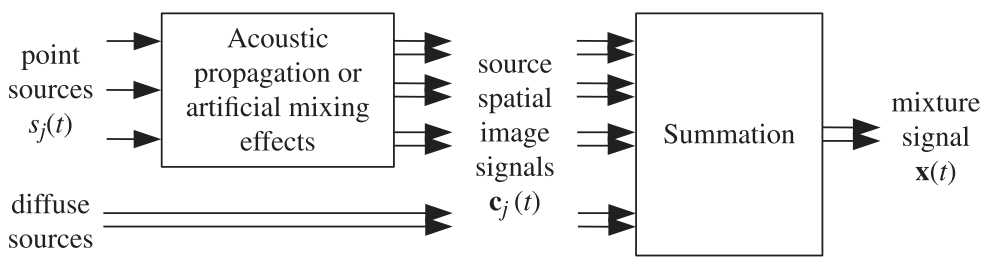
\includegraphics[width=\linewidth+\marginparsep]{processing/mixing_process.png}
    \end{fullwidthfig}

    \vspace{-\baselineskip}\vspace{-\baselineskip}
    \sideparmargin{outer}
    \sidepar{\vspace{\baselineskip}
    \caption{General mixing process, illustrated in the case of $\numSrcs = 4$ sources,
      including three point sources and one diffuse source, and $\numMics = 2$ channels.}
    }
    \label{fig:processing:mixing}
\end{figure}

In context of room acoustics and microphone recording, the mixing process is due to the propagation of sound in the auditory scene.
As discussed in~\cref{ch:acoustics:sec:wave}, this process is linear (and time invariant provided a static scenario).
% In this case, the spatialization operation $\spat_\idxSrc(\cdot)$ is expressed by
% collection of convolution with \RIR/ $h_{\idxMic\idxSrc}$
% from source $\idxSrc$ to microphone $\idxMic$ and the post-mixing operation $\master(\cdot)$ reduces to the identity:
\newthought{Therefore, we will model} the resulting mixture as the simple summation of the sound images,
which are the collections of convolution between the \RIRs/ and source signal:
\begin{align}
    \mics(t)         &= \sum_{\idxSrc=1}^{\numSrcs} \imgs_\idxSrc(t)\\
    \imgs_\idxSrc(t) &= \ktranspose{\klist{\img_{1\idxSrc}(t), \dots, \img_{\numMics\idxSrc}(t)}}\\
    \img_{\idxMic\idxSrc}(t) &=  \kparen{h_{\idxMic\idxSrc} \conv \src_\idxSrc} (t)
\end{align}
where $\conv$ is the linear convolution operator.

With the above notation, all the sources are threated in the same way, including \textit{target}, \textit{interfering} and \textit{noise} sources.
These definition depends on the specific use case, field of research and application.
Nevertheless, in speech processing context, it is common to refers to interfering and noisy sources as undesired speech \vs/ nonspeech sources respectively.

\subsection{Impulse Response Models}
Thanks to the convolution theorem, time-domain convolution can be implemented as a multiplication in the frequency-domain.
However this does not generalized straightforwardly to the time-frequency domain:
it depends on the length of the filter \wrt/ to the length of the analysis window on of the \STFT/.
Issues arise with long filter, which are common for microphone recoding in highly reverberant or time-varying scenarios.
To circumvent this issues, the \textit{convolutional STFT} with arbitrary analysis window have been proposed:
it implements the time-domain convolution into inter-time-frame and inter-frequency-bands products~\cref{aoe}.

In this thesis, we will assume that the filter length is much shorter than the analysis window length.
This known in the literature as the \textit{narrowband approximation}\cite{}.
\\In the time-frequency domain, $\mics_j(l,k)$  and $\src_j(l,k)$ are the \STFT/ of $\mics_j(l,k)$ and $\src_j(l,k)$ respectively.
Therefore, the time-domain filtering can be approximated by complex-valued multiplication in the STFT domain:
\begin{equation}
    \mics_j(l,k) = \bsh_j(k) \src_j(l,k)
    ,
\end{equation}
where the $\bsh_j(f) = \klist{h_{1j}(f), \cdots, h_{1j}(f)}$ is the $I \times 1$ vector of the DFT of the
\RIRs/ for the source $j$,

Recalling the derivation in~\cref{ch:acoustics:subsec:rir}, we adopt the following model for the room transfer function as:
\sidenote{\cfr{\cref{eq:acoustics:ims}}}
\begin{equation}
    \rir (k, \positionMicrophone \mid \positionSource) =
    ,
\end{equation}

\newthought{Steering Vector}
In case of absence of echoes and reverberation, namely assuming free-field propagation,
the \RIRs/ simplify to \textit{steering vector}, than is the DFT of~\cref{eq:acoustics:greenFreeTime}:
\begin{equation}\label{eq:processing:steering}
    \bsd_{j}(k) = \klist{\frac{1}{4 \pi \distMicSrc_{1j}} \cste^{-\csti 2 \pi f_k \distMicSrc_{ij} / c},
                            \cdots,
                            \frac{1}{4 \pi \distMicSrc_{Ij}} \cste^{-\csti 2 \pi f_k \distMicSrc_{Ij} / c},
                    }
\end{equation}
In far-field regimes, the microphone-to-source distance $\distMicSrc_{ij}$ are larger than the
inter-microphones distance $d_{ii'}$. Here the attenuation factors $\sfrac{1}{4 \pi \distMicSrc_{ij}}$ becomes approximately equal
and ofter are ignored.


\newthoughtpar{Relative Transfer Functions} modeled
Let us assume that the reference microphone is the first
The \RTFdef/:
\begin{equation}\label{eq:processing:rtf}
    \rtfs_j(k) = \frac{1}{\rir_{1j}(k)} \rirs_j(k)
\end{equation}

\newthought{Relative Steering Vectors} are under the free-far-field assumption on the sound propagation.
Interestingly from their closed form definition, an important geometrical property arise.
By combining~\cref{eq:processing:steering,eq:processing:rtf}, the \textit{relative steering vector} writes
\begin{equation}
    \bsd_{j}(k) = \klist{1,
                         \cste^{-\csti 2 \pi f_k \deltaTaus_{2j}},
                         \cdots,
                         \cste^{-\csti 2 \pi f_k \deltaTaus_{Ij}},
                    }
\end{equation}
where $\deltaTaus_{ij} = \frac{\distMicSrc_{ij}-\distMicSrc_{1j}}{c}$ is the \TDOAdef/.

\newthought{Interchannel Cues}
The \RTFs/ encodes the \ILDdef/ and the \IPDdef/
\begin{align}
    \ild_{ij}(k) &= 20 \log_{10} \magnitudeOf{\rtf(k)} \mathspace & [\si{\dB}]\\
    \ipd_{ij}(k) &= \phaseOf{\rtf(k)} \mathspace                  & [\si{\radian}]
\end{align}

As shown in ... the so-called \ILD/ and the \IPD/ cluster around the direct path. However early echoes and
reverberation make them significantly diverge.
\sidenote{%
    this terminology is used in the psycoacoustics fields
}


%%%%%%%%%%%%%%%%%%%%%%%%%%%%%%%%
\section{Audio Inverse Problems}
\cite{kitic2015cosparse}
\openepigraph{Their generality is of such a wide scope that onemayeven argue that solving inverse problems is what signal processing is all about}{Srdan Kiti\'c, \textit{Cosparse regularization of physics-driven inverse problems}}
\openepigraph{everything is an optimization problem}{\citeonly{watson2001nonlinear}}
\marginpar{
    \footnotesize
    One can see the paralelism with the engineering concepts: analysis and sythesis.
}
In~\cref{sec:intro:problem} we have informally defined \textit{inverse problems}, with an emphasis on inverse problems in signal processing.
An inverse problem is a type of a mathematical problem where we start with the observations and we want to estimate model parameters that produced them.
\\Inverse problems pervades all the field of science and engineering:
source localization~\cite{},
image processing~\cite{},
acoustic imaging and tomography~\cite{},
\marginpar{
    \footnotesize
    A historical example are the calculation of the Earth circunference by Eratosthenes in III century b.c.\\
    and the calculations of Adams and Le Verrier which led to the discovery of Neptune from the perturbed trajectory of Uranus.
}

A inverse problems is defined as the counterpart of a \textit{forward}\sidenote{often referred to as \textit{direct}} problem.
Without falling in and deep mathematical formalism and taxonomies which can be found in \citeonly{bal2012introduction},
we will simply consider the following informal definition:
\begin{center}
    \textit{\emph{Forward problem} starts from known input, while \emph{inverse problem} starts from known output~\cite{santamarina2005discrete}.}
\end{center}
Both these problems focus on an operation relating maps objects of interest, called \textit{parameters} or \textit{variables},
to information collected about these objects, called \textit{measurements}, \textit{data} or \textit{observation}.

For instance, in our context, the direct problem may be the estimation of the \RIR/(s) starting from the known room parameters,
and, the related inverse problem would be the estimation of such room properties from the observation of the \RIR/(s).

Formally, a forward problem is defined through a mathematical model, described by a \textit{operation} $\scrM(\cdot)$
mapping \textit{parameters} $x \in \scrX$ to the \textit{observation} (or measurement) $y \in \scrY$:
\begin{equation}\label{eq:processing:model}
    y = \scrM(x)
    .
\end{equation}
Then, the inverse problem defines a method $\kinv{\scrM}$ that ``reverts'' $\scrM$ in order to recover (estimate) $x$ form the observation of $y$.
% The operator $\scrM$ describes our best effort to construct a \textit{model} for the available data $y$.
% The choice of $\scrX$ describes our best effort to characterize the space where we believe the parameters belong.

As discussed in~\cite{bal2012introduction}, \textit{solving} the inverse problem consists in finding point(s) $x \in \scrX$ from (knowledge of) data $y \in \scrY$
such that~\cref{eq:processing:model} or an approximation of~\cref{eq:processing:model} holds.
Under this light, the operator $\scrM$ ant the choice of $\scrX$ describes our best effort to construct a \textit{model} for the data $y$ and
the space where the parameters $x$ belong, respectively.
\marginpar{
    \footnotesize
    one can already see the paralelism the the definition of the mixing process defined in~\cref{sec:intro:problem}
}

\textsc{For instance, in Case of} \textit{linear} inverse problem, and for $\scrY$ and $\scrX$ being vector spaces of dimensions $M$ and $N$ respectively,
then the forward map can be written as a linear system:
\begin{equation}\label{eq:processing:linear_forward}
    \bfy = \bfM \bfx
\end{equation}
where $\bfM$ being a matrix, namely the operator $\scrM$ becomes a matrix multiplication by $M$.
It follows that the inverse map associated to~\cref{eq:processing:linear_forward} is the application of the inverse matrix $\kinv{M}$.
% While solving a direct problem the an operator needs to be found, in solving the inverse one either the operator is known and needs
% to be $reverts$t

Typically, forward problems are considered somehow the ``easier''.
In fact, even in the observation model $\scrM$ is known perfectly, it is not always possible to find its counterpart.
This because of
\begin{itemize}
    \item presence of \textit{noise} in the measurement which are not always additive and statistically independent \wrt/ $x$.
    \item the problem is \textit{well-posed} and \textit{well-conditioned}, namely $\scrM$ needs be injective and stable.
    In other words, some information is recoverable, other is completely lost, other highly sensible to noise
    \sidenote{
        \textbf{injective} ensure the uniqueness of the solution, while \textbf{stability}
        ensure a continuity on the data.
        These are known as the Hadamard's \textit{solvability conditions}.
    }.
\end{itemize}

As we could images, many interesting and fundamental inverse problem are
\textit{ill-posed} or \textit{ill-conditioned} in general, even in the following ``simple'' ones~\cite{kitic2015cosparse}:
The solution to the deconvolution problem, where the direct inversion of the transfer function results in instabilities
at high frequency; and the solution a linear system $\bfy = \bfM \bfx$ where $\bfM$ is invertible
may lead to erroneous results and numerical instabilities.

Therefore, sometimes ones have to settle for restring the set of solution $\scrC \subset \scrX$,
where $\scrM$ is stable and injective\sidenote{This framework was originally proposed by Tikhonov.}.
Promoting solution $x \in \scrC$ is can be achieved through \textit{model priors}, namely prior knowledge about solution, which can
be classified in the following methodologies:
the usage of \textit{geometric constraints} that deterministically define the solutions; the imposition of \textit{penalization}
which ``promotes'' solution of a certain shape (\eg/ \textit{sparse}
\sidenote{\textbf{sparsity} is a fundamental concept of this thesis, better discussed in~\cref{pt:estimation}
} or \textit{smoothness});
and casting the problem in a \textit{bayesian framework} which versatilely incorporate prior and posterior density function describing the data.

\subsection{General Processing Scheme}
Digital signal processing (DSP) is the process of analyzing and modifying a signal to optimize or improve its efficiency or performance. It involves applying various mathematical and computational algorithms to analog and digital signals to produce a signal that's of higher quality than the original signal.
It is traditional in engineering to represent complex systems as a collection of simpler subsystems, with well-defined tasks, interacting with each other.
In signal processing, these subsystems roughly fall into four categories: \textit{representation}, \textit{enhancement}, \textit{estimation}, and \textit{adaptive processing}.
Many problems can be decomposed into blocks that belong to one of these categories.

\begin{description}
    \item[Representation] Objects can be represent (described) in many different way.
    Through different representations, some object \textit{information} becomes more relevant and suitable for certain tasks
    than other.
    \\Representation can be lossy or lossless, and are generally implemented through (non)linear mapping, such as change of basis or feature.
    The most famous representation is the Fourier basis.
    \\Depending on the task the representation may be invertible.
    The process of changing representation is often called: Analysis and Synthesis

    \item[Enhancement] Measurement are affected by noise and interferences which corrupt and hide relevant information, making inverse problems ill-posed and ill-conditioned.
    Therefore, signal enhancement, that is removing noise, is a necessary step.
    \\Enhancement constitute a huge dome of methods: form simple denoising by averaging of repeated measurement to
    spectral subtraction to source separation with neural network.

    \item[Estimation] Often we wish to estimate some key properties of the target signal which may be used as inputs to a different algorithm.

    \item[Adaptive processing] deals with adaptive algorithms and filters controlled by variable parameters.
    A common means to adjust those parameters according to an optimization algorithm which rely on statistical properties of the signal of interest.
    They often implement a kind of online optimization where an objective function is being minimized.
    When new data is observed, its discrepancy with the current estimate is used to produce a new estimate in a way that reduces the objective.
\end{description}

Let us give two example of practical systems that will be recurrent thought out the entire thesis.

\subsection{Selected Audio Inverse Problems}
Here follow some famous problems in the field of audio signal processing with application to speech, music and environmental audio.
Given the mixing process defined in~\cref{sec:processing:model},

% \begin{description}
%     \item[sound source separation and enhancements] as the problem of retrieving a (set of) source signal from a mixture.
%     \item[sound source localization] estimation of source location from the observation of the sound production.
%     This has sense as long as the impulse response convey space properties.
%     \item[microphones calibration] estimation of the microphone placement.
%     \item[\RIR/ estimation] estimation of the filters.
%     Blind Channel Estimation or System Identification.
%     \item[Acoustic Echoes Estimation] estimation of the filters
%     \item[dereverberation] estimation of the filters
%     \item[room geometry estimation] estimation of the room
%     \item[automatich speech recognition]
% \end{description}

\begin{table}[!h]

    \begin{fullwidthfig}
    \centering
    \small

    \begin{tabular}{p{0.33\linewidth}|p{0.66\linewidth}}
        \toprule
        Inverse Problem & \textit{Can we estimate the...} \\
        \hline
        Audio Source Separation  & the signal of the sources $s_{j}$ from the mixture $\boldsymbol{x}$? \\

        Sound Source Localization & the position $\mathbf{s}_{j} \ =\ [ x_{s_{j}} ,\ y_{s_{j}} ,\ z_{s_{j}}]$  of the source $s_{j}$ from the mixture $\boldsymbol{x}$$ $? \\

        Microphone (Array) Calibration & the position of the microphone (array) position $\mathbf{x}$ from the mixture $\boldsymbol{x}$? \\

        \RIR/ Estimation & the filter between the sources $\boldsymbol{s}_{j}$ and the mixture $\boldsymbol{x}$ from $\boldsymbol{x}$? \\

        Room Geometry Estimation & the shape of the room in which the mixture $\boldsymbol{x}$ recoding source $s_{j}$? \\
        \bottomrule
    \end{tabular}

    \end{fullwidthfig}

    \vspace{-\baselineskip}\vspace{-\baselineskip}
    \sideparmargin{outer}
    \sidepar{\vspace{\baselineskip}
        \caption{Selected audio inverse problems}
    }
    \label{tab:processing:problems}


\end{table}

\openepigraph{Everything is connected}{Douglas Adams, \textit{Dirk Gently's Holistic Detective Agency}}
\newthought{Depending on the scenario}, all these problems exhibits strong inter-connections,
namely the solution of one may be (dependent on) the solution of another.
Therefore, exploiting expertise and knowledge,
interconnect and hierarchical approaches may be built\sidenote{Machine Learing allows now for end2end approaches}:
for instance, many spatial filtering techniques used for \SE/ rely on \SSL/ blocks;
and in order to achieves \RooGE/, \AER/ must be done.

\section{Time, Frequency and Time-Frequency Audio Signals}
The raw \textit{audio signal} encodes the variation of pressure over time on the microphone membrane.
Mathematically it can be written as the the \textit{measure}\sidenote{measure, function, operator}
$x$ continuous both in time $t \in \R$ and in amplitude $x(t) \in \R$.
\\Today signals are processed, stored and analyzed by computer and digital modules in their
digital representation.
In short, the \textit{digital audio signal} is obtained from an analog signal in two steps:
first, the continuous time signal $x(t)$ is converted to a discrete time series,
so that one sample\sidenote{
   Please note, that the use of the word \textit{sample} will have different
   meanings in the context of machine learning, where a sample is an instance of a full signal instead of a single time
} $x(n)$ with $n \in \Z$ is \textit{sampled} with equidistant steps $\Ts$;
second, the amplitude values can be \textit{quantized}.
At the end of the digitalization process, $x(n) \in \R$ with $n = 0, \dots, N-1$, represents a one dimensional time series of amplitudes.
\\An important parameter in the process of digitization is the \textit{sampling frequency},  $\Fs = \sfrac{1}{\Ts}$
where $\Ts$ is the sampling period.
The choice of $\Fs$ depends massively on the application since it translates into a trade-off between computational power, sound and processing quality.
Historically two iconic values are $\SI{44.1}{\kHz}$ for music distribution on CDs and $\SI{8}{\kHz}$ for first-generation speech communication.
Now multiple of $\SI{8}{\kHz}$ are typical chosen values: ($16, 48, 96, \SI{128}{\kHz}$).
\\For further details, we refer the reader to audio signal processing basics books such as~\cite{rocchesso2003introduction}.

\newthought{The Frequency Representation}, \aka/ \textit{spectral representation}, is probably the most famous signal representation used in signal processing.
It was introduced by Joseph Fourier in his work on the heat equation~\cref{baron1822theorie}.
He proposed a mathematical tool, named later \textit{Fourier Decomposition}, aiming at approximating any signal by a sum of sine and cosine waves.
Speech and music signals, naturally exhibits harmonic and periodic behaviors, are well described
by combination of sinusoids as function of their frequencies.

The (forward) \FTdef/ of the continuous time domain signal $x$:
\begin{equation}
    x(f) = \fourierTrans{x}(f) =
        \int_{-\infty}^{+\infty}
        x(t)
        \cste^{-\csti 2 \pi f t}
        \,\kdiff{t}.
\end{equation}
where $f \in \kintervoc{-\sfrac{\Fs}{2}}{\sfrac{\Fs}{2}}$ are the \textit{natural frequency} in $\si{\Hz}$ and $\csti$ is the imaginary unit.

The (forward) \DFTdef/ of the discrete-time domain signal $x$:
\begin{equation}\label{eq:processing:dft}
    x(k) = \discreteFT{x}(k) =
    \sum_{n = 0}^{2 N - 1}
    x(n)
    \cste^{-\csti2\pi \tfrac{k n}{2 F}}.
\end{equation}
with $k \in \kintervcc{0}{2 F - 1}$.

We denote the frequency in $\si{\Hz}$ associated with the frequency bins $k = 0, \cdots, $ as:
\begin{equation}
    f = \frac{k}{F}\Fs.
\end{equation}

A raw audio signal encodes the amplitude of a sound as a function of time; while, its Fourier spectrum
represents it as a function of frequency, but los completely variation over time.
In order to jointly account for temporal and spectral characteristic, following representation is used.

\newthought{\TFdef/ Representation} aims to jointly describe the signal in time and frequency domain.
the \STFTdef/ It encodes the time-varying spectra into a matrix $x(k,l) \in \bbC^{F,T}$ with frequencies $k$ and time frames $l$.

the \STFT/ has the following useful properties for audio processing~\cite{vincent2018audio}:
\begin{itemize}
    \item the frequencies scale $f$ is a linear function of the frequency bin $k$;
    \item the resulting matrix allows easy treatment of
          the phase $\phaseOf{x(k,l)}$, the magnitude $\magnitudeOf{x(k,l)}$ and the power $\powerOf{x(k,l)}$ separately;
    \item the \DFT/ can be efficienciently computed with the \FFT/ algorithm;
    \item the \STFT/ is simple to invert.
\end{itemize}

\newthoughtpar{Time-Frequency Analysis, Processing and Synthesis}
Throughout this dissertation both estimation and processing will be conducted in the  \TF/ domain.
This is a common approach in the audio signal processing community, but it is not the only one:
Many algorithm are designed directly in the time domain.
\\Along with common motivation supported by time-domain resolution or computational load requirements,
powerful machine-learning approaches are able to learn both representation and estimation steps~\cref{subsec:application:algos}.
\\In the context of \STFT/, the process of converting the signal into the \TF/-domain is called \textit{analysis}, while
its counterpart converting back to time-domain is called \textit{synthesis}.
Between the two we will conduct \textit{estimation}, \textit{processing} and \textit{enhancement}.
\\The \STFT/ Analysis, \STFT/ Synthesis

%%%%%%%%%%%%%%%%%%%%%%%%%%%%%%%%
\section{Taxonomy through dichotomies}
\cite{vincent2018audio}

%% acoustics %%
\newthoughtpar{Sources \vs/ Mixtures}
Sound sources emits sounds.
When multiple sources are active at the same time, the sound that reaches our ears or is recorded using a microphone is superimposed or \textit{mixed} to a single sound.
A \textit{mixture} represents a mapping from a set of sources $s$ to an output signal $x$.

\newthoughtpar{Single-Channel \vs/ Multichannel}
A \textit{single-channel} signal ($\numMics = 1$) is represented by the scalar $\mic(t) \in \R$,
while a \textit{multichannel} ($\numMics >   1$) is represented by the vector

\newthoughtpar{Point \vs/ Diffuse Sources}
\textit{Point sources} are emitted by a single and well-defined point in the space $\positionSource_\idxSrc$ and their signal is single channel.
Point sources are for instance human speakers or the sound emitted by a loudspeaker.
\\\textit{Diffuse sources} refers for instance to wind, traffic noise, or large musical instruments, which emit sound in a large region of space.
Their sound cannot be associate to a punctual source, but rather a distributed (infinite) collection of them.

\newthoughtpar{Directional \vs/ Onmidirectional Sources and Receiver}
An \textit{omnidirectional} source (\resp/ receiver) will in principle emit (\resp/ pick up) sound equally from all directions,
with respect both time and frequency.
Although this simplify greatly processing frameworks, this is not true in real scenario.
The physical properties of real sources (\resp/ receivers) leads to \textit{directivity patterns} which may
be different at different frequencies.
This effect may be a source of undesired effects, such as microphones \textit{leakage} or source localization error.
Nevertheless sometimes it can be exploited to promote \textit{spatial selectivity}:
spatial filtering can be view under this light, where ``virtual'' microphones with engineered directivity pattern.


%% processing %%
\newthought{Linear \vs/ Non-linear}
If the whole mixing (and mastering) processes is \textit{linear}, and \textit{non-linear} otherwise.

\newthoughtpar{Natural \vs/ Artificial Mixtures}
Natural mixture, or Microphone recordings, refer to the situation when multiple sources which are simultaneously active are captured by a microphone array.
Typical examples include hands-free phones, audio conferencing systems, and hearing aids.
Artificial mixtures, by contrast, are generated by mixing individually recorded sound sources using appropriate hardware or software. Most audio media (television, music, cinema, etc.) fall into this category

\newthoughtpar{Instantaneous \vs/ Convolutive Mixtures}
For instantaneous mixtures, all sources are mixed using fixed mixing parameters aj.
This is the typical scenario when sources are mixed using a mixing console.
In convolutive mixtures, each source sj is convolved by a filter response rj before summation
Usually, the mixing process is assumed to be time-invariant but for
a variety of signals, such as live recordings with moving sources, it can also be time-variant. The mathematical notations of different mixing models are summarized in Table 2.2.

\newthoughtpar{White Gaussian \vs/ Babble Noise}
White noise

\newthoughtpar{Measurements \vs/ Diffuse Noise}
\begin{center}
    \textit{\emph{Noise} is a general term for unwanted (and, in general, unknown) modifications that a signal may suffer during capture, storage, transmission, processing, or conversion}
    ~\cref{tuzlukov2018signal}.
\end{center}
Modeling noise is important in context of signal processing as it accounts for all the unwanted or unknown effects:
it may refer to undermodeling (residual) errors, undesired sound sources, \etc/.
In the context of audio inverse problem, it is common to model noise as an additive error term following a Gaussian distribution:
\begin{equation}\label{eq:processing:model}
    y = \scrM(x) + \error \mathspace \error \text{with} \; \sim \calN(0, \sigma^2)
\end{equation}
In this thesis, we will refer to this type noise as \textit{measurement noise}, as it corrupts the observed (\ie/ measured) data,
and it is modeled as white (\ie/ spectrally flat) Gaussian noise, which is the basic noise model used in signal processing to mimic the effect of many random processes that occur in nature.
\\When comes to microphones recordings, environmental noise is diffuse with